% !TeX spellcheck = it

\documentclass{article}

\usepackage{makeidx}
\usepackage{natbib}
\usepackage{amsthm}
\usepackage{mathtools}
\usepackage{algorithm}
\usepackage{algpseudocode}
\usepackage[T1]{fontenc}
\usepackage[utf8]{inputenc}
\usepackage[italian]{babel}
\usepackage[a4paper, total={6in, 8in}]{geometry}
\usepackage{parallel,enumitem}
\usepackage{graphicx}
\usepackage{float}
\usepackage[%  
    colorlinks=true,
    pdfborder={0 0 0},
    linkcolor=black
]{hyperref}

\makeindex
\title{Analisi sensitività}
\author{Niccolò Kadera}
\date{\today}
\newtheorem{example}{Esempio}


\begin{document}
{\fontfamily{lmss}\selectfont
\maketitle

\section{Parametri e valori di default}

\subsection{Valori di default e spiegazione parametri}
Di seguito vengono spiegati tutti i parametri del modello, e tra parentesi quadre viene inserito il valore default: \newline

    \textbf{Parametri della simulazione}
    \begin{itemize}
        \item \textbf{$T$ (max\_days):} [100] Numero di giorni per ogni simulazione.
        \item \textbf{$n$ (n\_persons):} [2000] Rappresenta il numero di persone per ogni simulazione.\newline
    \end{itemize}

    \textbf{Parametri sociali}
    \begin{itemize}
        \item \textbf{$b_{c}$ (capacity):} [1500] Questo numero intero rappresenta la capacità massima della barra (è u utile se respect\_the\_max: bool = True).
        \item \textbf{$t_a$ (threshold): } [0.5] Questa soglia viene utilizzata per determinare se un agente andrà al bar o meno a seconda della sua strategia.
        \item \textbf{respect\_the\_max: } [True] Questo booleano rappresenta se la capacità della barra sarà rispettata o meno..\newline
    \end{itemize}

    \textbf{Strategie degli agenti}
    \begin{itemize}
        \item \textbf{strategyOne:} [0.1] Percentuale sul totale degli agenti che seguiranno la strategia uno per l'ottenimento della prima decisone riguardo alla presenza al bar. La prima strategia è totalmente randomica.
        \item \textbf{strategyTwo: } [1 - strategyOne = 0.9] Percentuale sul totale degli agenti che seguiranno la strategia due per l'ottenimento della prima decisone riguardo alla presenza al bar. La seconda strategia è calcolata parzialmente con una regressione lineare del vettore memoria contenente le precedenti strategie degli agenti.
        \item \textbf{useRegrFrom: } [10] Indica il giorno dal quale gli agenti che seguono la strategia due potranno utilizzare una regressione lineare, in quanto il vettore memoria sarà sufficientemente popolato.
        \item \textbf{useRegrFor: } [1] Dell'output totale della strategia definita dall'agente ogni settimana, il valore definito dalla regressione lineare delle precedenti influisce su una percentuale definita dal parametro.\newline
    \end{itemize}

    \textbf{Parametri epidemiologici}
    \begin{itemize}
        \item \textbf{num\_infected\_persons:} [100] Identifica il numero di persone contagiose ad inizio simulazione.
        \item \textbf{$t_{c}$ (infection\_threshold):} [0.4] Un'altro agente diventa contagioso se il suo livello contagio $c_{j}$ è maggiore del contagious\_threshold. Quindi se un agente ha un livello di contagio inferiore a $t_{c}$ non potrà più infettare altri agenti.
        \item \textbf{$t_{s}$ (infection\_thresholdNotPresent):} [0.8] Per cui se un agente ha un livello di contagio $c_{j}$ maggiore di $t_{s}$ allora, indipendentemente dal valore di della stategia, non si presenterà al bar in quanto i sintomi dell'infezione sono troppo elevati.
        \item \textbf{$t_{i}$ (infection\_duration):} [10] Identifica la durata in giorni dell'infezione, senza
        \item \textbf{$t_{r}$ (infection\_cantStartUntil):} [2] Dopo che un agente guarisce da un infezione, il valore identifica quanto tempo un agente è immune ad una nuova infezione.
        \item \textbf{infection\_generatesResistance:} [True] Abilita il valore precedente, per l'agente deve attendere $t_{r}$ giorni, dopo essere guarito, per essere infettato nuovamente
        \item \textbf{people\_memory\_weight\_arr:} [[0.5, 0.2, 0.1]] Pesi relativi assegnati alla memoria delle precedenti strategie salvate nel vettore memoria. In questo caso, l'ultimo valore inciderà per un 50\% sul valore finale della strategia, il penultimo 20\%, il terzultimo 10\% ed il rimanente 20\% verrà ripartito tra tutti gli altri valori presenti nel vettore memoria.
        \item \textbf{$\alpha$ (alpha):} [0.2] Peso che varia il numero di nuovi infetti per agente.
        \item \textbf{regression\_type:} [1] Grado della regressione effettuata con np.polyfit (1 = regressione lineare).
        \item \textbf{infection\_randomness:} [0.25] Altera il livello di contagio per un valore randomico che spazia tra -infection\_randomness e +infection\_randomness.\newline
    \end{itemize}
    
    \textbf{Parametri del Policy Maker}
    \begin{itemize}
        \item \textbf{enablePM:} [True] Abilita il Policy Maker nella simulazione.
        \item \textbf{enableA1 :} [True] Abilita la strategia A1 del PM. Ovvero l'azione per cui viene ridotta la capacità massima del bar.
        \item \textbf{enableA2 :} [True] Abilita la strategia A2 del PM. Ovvero l'azione per cui viene imposto l'utilizzo di mascherine all'interno del bar.
        \item \textbf{enableA3 :} [True] Abilita la strategia A3 del PM. Ovvero l'azione per cui viene effettuato un test sul livello di contagio all'entrata del bar.
        \item \textbf{enable\_at\_least\_one\_A :} [False] Limita il PM ad abilitare una sola azione, ha effetto quando il reinforcement learning è diabilitato o nella modalità 2.
        \item \textbf{$\delta$ (delta):} [150] Costo per ogni nuovo infetto
        \item \textbf{$r_{i}$ (r):} [0] Ricavo per ogni agente, viene utilizzato in realzione al numero dei guariti ad ogni istante di tempo.\newline
    \end{itemize}

    \textbf{Parametri Azione 1}
    \begin{itemize}
        \item \textbf{$r_{a1}$ (a1\_reductionPerc):} [0.8] È la percentuale di riduzione della capacità massima dela bar nel momento in cui A1 è attiva.
        \item \textbf{a1\_reductionDuration :} [10] Durata dell'azione A1 per la modalità uno del reinforcement learning o reinforcement learning disattivato.
        \item \textbf{a1\_InfectedTreshold :} [0.375] Per le simulazioni con reinforcement learning disattivato viene utilizzato per definire quando attivare la strategia A1, ovvero quando il numero di infetti totali supera $n \cdot a1\_InfectedTreshold$.
        \item \textbf{$\alpha_{1}$ (a1\_cost):} [2] Rappresenta il costo dell'azione A1, esso viene moltiplicato per il numero di infetti totali ogni istante in cui l'azione rimane attiva.\newline
    \end{itemize}

    \textbf{Parametri Azione 2}
    \begin{itemize}
        \item \textbf{$m1_{a2}$ (a2\_faceMask1Agents):} [0.65] Percentuale di agenti che indosseranno la mascherina di tipo 1.
        \item \textbf{$m2_{a2}$ (a2\_faceMask2Agents):} [0.3] Percentuale di agenti che indosseranno la mascherina di tipo 2.
        \item \textbf{$m0_{a2}$ (a2\_faceMask2Agents):} [0.05] Percentuale di agenti che indosseranno la mascherina di tipo 0, ovvero coloro che riusciranno ad entrare nel bar senza l'utilizzo di una maskerina.
        \item \textbf{$mp1_{a2}$ (a2\_faceMask1Perc):} [0.3775] Aumento del threshold di contagio $t_{c}$ per gli agenti che utilizzano la mascherina di tipo 1.
        \item \textbf{$mp2_{a2}$ (a2\_faceMask2Perc):} [0.5] Aumento del threshold di contagio $t_{c}$ per gli agenti che utilizzano la mascherina di tipo 2.
        \item \textbf{a2\_reductionDuration :} [1] Durata dell'azione A2 per la modalità uno del reinforcement learning o reinforcement learning disattivato.
        \item \textbf{a2\_InfectedTreshold :} [0.1] Per le simulazioni con reinforcement learning disattivato viene utilizzato per definire quando attivare la strategia A2, ovvero quando il numero di infetti totali supera $n \cdot a1\_InfectedTreshold$.
        \item \textbf{$\alpha_{2}$ (a2\_cost):} [8] Rappresenta il costo dell'azione A2, esso viene moltiplicato per la capienza del bar ogni istante in cui l'azione rimane attiva.\newline
    \end{itemize}

    \textbf{Parametri Azione 3}
    \begin{itemize}
        \item \textbf{a3\_testFailUnder:} [0.45] Percentuale di errore del test.
        \item \textbf{a3\_reductionDuration :} [1] Durata dell'azione A2 per la modalità uno del reinforcement learning o reinforcement learning disattivato.
        \item \textbf{a3\_InfectedTreshold :} [0.2] Per le simulazioni con reinforcement learning disattivato viene utilizzato per definire quando attivare la strategia A3, ovvero quando il numero di infetti totali supera $n \cdot a1\_InfectedTreshold$.
        \item \textbf{$\alpha_{3}$ (a2\_cost):} [25000] Rappresenta il costo dell'azione A3, esso rappresenta un costo fisso e viene contabilizzato solo la prima volta che viene seguita A3.\newline
    \end{itemize}

    \textbf{Reinforcement Learning PM}
    \begin{itemize}
        \item \textbf{enableRL:} [True] Abilita il reinforcement learning per il Policy Maker.
        \item \textbf{RL\_mode:} [2] Definisce la modalità di reinforcement learning, la modalità 1 ha come ipotesi la possibilità di attivare una azione per volta, mentre la modalità 2 consente l'attivazione di più strategie simultaneamente unificandone il tempo di attivazione (reductionDuration).
        \item \textbf{a\_reductionDuration:} [15] Tempo di attivazione (reductionDuration) attribuito a tutte le strategie nel caso di RL\_mode = 2.
        \item \textbf{$\epsilon_{RL}$ (epsilon\_RL):} [0.2] Percentuale di esplorazione del PM, al crescere di $\epsilon_{RL}$ il PM esplorerà meno affidandosi maggiormente a già quanto salvato nella q-table. Nelle simulazioni ad epoche viene applicato l'epsilon greedy algorithm.
        \item \textbf{$\alpha_{RL}$ (alpha\_RL):} [0.3] Percentuale per cui viene aggiornato il valore salvato in q-table, con $\alpha_{RL} = 1$ viene rimpiazzato il valore precedente salvato in q-table.
        \item \textbf{$t_{minPm}$ (RL\_PM\_t\_min):} [15] Tempo minimo per il quale il PM non si attiverà, esso entrerà in azione dopo RL\_PM\_t\_min giorni.
        \item \textbf{infection\_slope\_regr\_len:} [5] Per definire lo stato nel quale si trova il PM, viene effettuata una regressione lineare degli ultimi infection\_slope\_regr\_len giorni ed estrapolata la pendenza dallo storico delle infezioni.
    \end{itemize}

\subsection{Simulazioni con parametri di default}
\begin{figure}[H]
    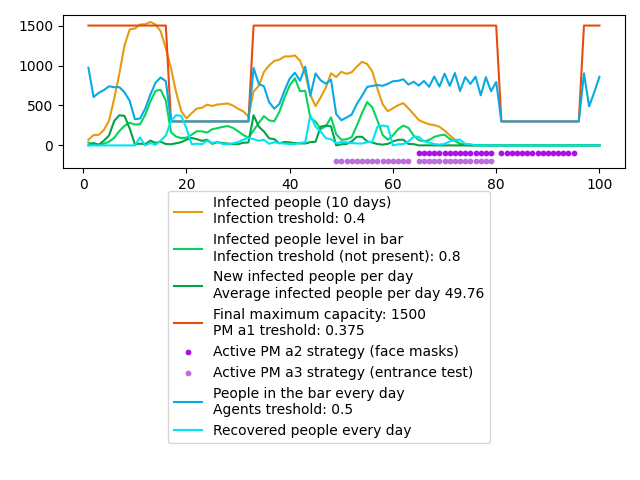
\includegraphics[width=\linewidth]{media/d_1_2.png}
    \caption{Simulazione 1 default (/media/d\_1\_2)}
    \label{fig:d_1_2}
\end{figure}
\subsection{Simulazioni con parametri di default}
\begin{figure}[H]
    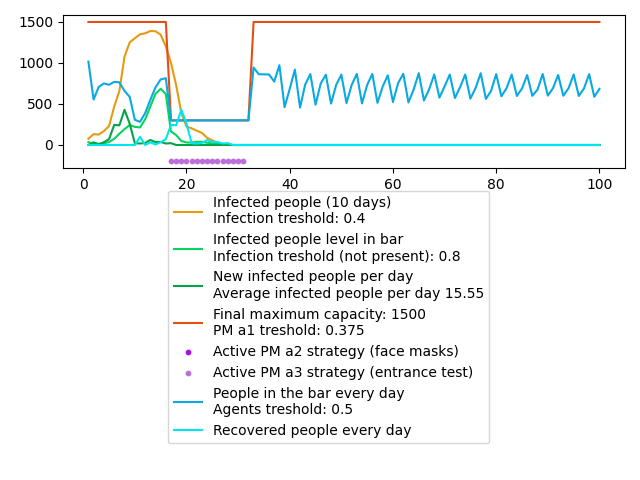
\includegraphics[width=\linewidth]{media/d_1_198.png}
    \caption{Simulazione 198 default (/media/d\_1\_198)}
    \label{fig:d_1_198}
\end{figure}
\begin{figure}[H]
    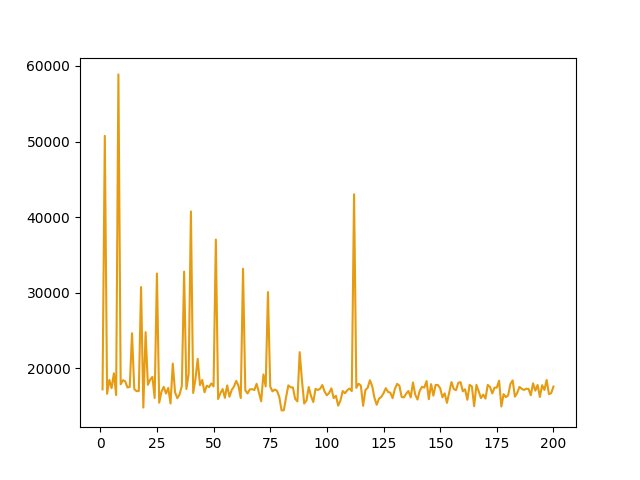
\includegraphics[width=\linewidth]{media/d_1_infection.png}
    \caption{Infection default (/media/d\_1\_infection)}
    \label{fig:d_1_infection}
\end{figure}
I parametri default dimostrano il corretto funzionamento del modello. Il PM inizia con un contagio che si protrae a lungo nell'epoca (Figure\ref{fig:d_1_2}), raggiungendo poi uno stato in cui riesce efficacemente ad interromperlo, azionando le strategie corrette (Figure\ref{fig:d_1_198}).\newline
Il corretto funzionamento viene confermato anche dal grafico che mette in relazione il numero dei contagi per epoca con l'id dell'epoca stessa (Figure\ref{fig:d_1_infection}). Si può notare come avvicinandosi all'epoca finale (200) il numero di contagi tenda ad un intorno di 1500 per epoca.\newline
Il Policy Maker ha identificato come azioni per eliminare il contagio una combinazione tra A1 ed A2 attivate subito dopo il $t_{minPm}$.



\section{Analisi parametri}

In questa analisi verranno studiati i seguenti paramteri del modello: $\delta$, $t_{a}$, $r_{a1}$, $c_{a2}$, $c_{a3}$.

\subsection{Analisi $c_{a3}$}
\subsubsection{$c_{a3} = 40000$}
Una prima analisi effettuata è stata quella di aumentare il costo dell'azione 3, ovvero $c_{a3}$, a 40.000. Questo valore è stato scelto in quanto non molto elevato, e si è voluto studiare l'effetto che avrebbe avuto sulle azioni del PM. \newline
\begin{figure}[H]
    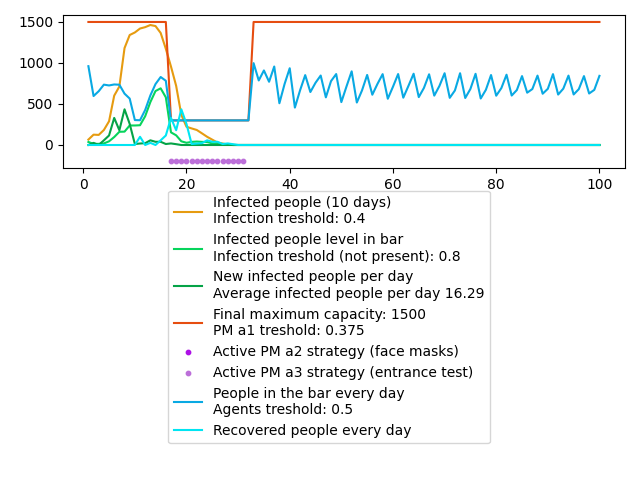
\includegraphics[width=\linewidth]{media/a3_c_40000_198.png}
    \caption{Simulation 198 a3 cost 40.000 (/media/a3\_c\_40000\_198.png)}
    \label{fig:a3_c_40000_198}
\end{figure}

Notiamo come a fine epoca il PM abbia attivato le azioni 1 e 3, nonostante il costo dell'azione 3 fissato a 40.000. Nella simulazione 198 (Figure\ref{fig:a3_c_40000_198}) il PM riesce al giorno 29 a fermare il contagio con la combinazione di azioni scelta, il risultato viene ritenuto accettabile considerando i 15 giorni iniziali in cui il PM non può attivare nessuna azione e la media di infetti per ogni gionro a 16,29.

\subsubsection{$c_{a3} = 50000$}
Viene continuato ad aumentare il costo dell'azione 3, arrivando ad un valore di 50.000. \newline
\begin{figure}[H]
    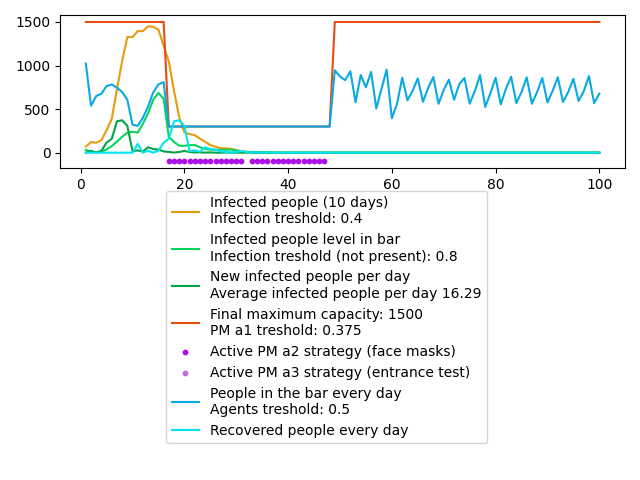
\includegraphics[width=\linewidth]{media/a3_c_50000_200.png}
    \caption{Simulation 198 a3 cost 40.000 (/media/a3\_c\_50000\_200.png)}
    \label{fig:a3_c_50000_200}
\end{figure}

\printindex

\bibliographystyle{plain}
\bibliography{mybib.bib}

}
\end{document}